\documentclass{article}
\usepackage{iclr2027_conference,times}
\input{math_commands.tex}
\usepackage{amsmath,amssymb,amsthm,mathtools}
\usepackage{booktabs,array,multirow}
\usepackage{capt-of}
\usepackage{graphicx}
\usepackage[dvipsnames]{xcolor}
\usepackage{tikz}
\usetikzlibrary{arrows.meta,positioning,fit,calc}
\usepackage{enumitem}
\usepackage{microtype}
\usepackage{hyperref}
\usepackage{url}
\hypersetup{hidelinks}

\title{When Should an Agent Return?\\Reliable Resource-to-Go under Closed-Loop Composition Shift}
\author{Anonymous authors\\Paper under double-blind review}

\newtheorem{theorem}{Theorem}
\newtheorem{proposition}[theorem]{Proposition}
\newtheorem{corollary}[theorem]{Corollary}
\newtheorem{remark}{Remark}
\newcommand{\RtoGo}{\mathcal{E}_{C}}
\newcommand{\trueR}{U}
\newcommand{\predR}{\widehat U}
\newcommand{\continueaction}{\textsc{Continue}}
\newcommand{\returnaction}{\textsc{Return}}
\newcommand{\resultpending}[1]{\textcolor{BrickRed}{\textbf{[RESULT PENDING: #1]}}}
\newcommand{\evidencepending}[1]{\textcolor{RoyalBlue}{\textbf{[EVIDENCE SLOT: #1]}}}

% Keep commented for anonymous submission.
% \iclrfinalcopy
\begin{document}
\maketitle
\begin{abstract}
When should a resource-limited agent stop working and commit to replenishment? Returning too early sacrifices throughput, but returning too late risks stranding, and neither state of charge nor geometric distance captures the future trajectory produced by a learned policy composed with a hard safety operator. We study charger Resource-to-Go under this compositional closed-loop shift. The key distinction is between pair novelty and executed-interface extrapolation: an unseen policy--operator pair can remain identifiable when its target executed interface is covered, whereas behavior outside that support is not identifiable without additional structure. We pair this identification boundary with an assumption-explicit account of long-horizon error accumulation and a decision-stability result that confines decision changes from bounded prediction error to a band around the return boundary. Our framework uses executed-interface Resource-to-Go estimates in an irreversible ReturnManager, adds epistemic margins or abstention only when justified, and leaves collision safety to the hard operator. \resultpending{ORACLE HEADROOM; PAIR VS. INTERFACE; FINAL RETURN PARETO} The planned evaluation tests whether this view predicts failure across controlled policy--operator compositions and improves the stranding--throughput frontier beyond simple heuristics, direct switching, world-model ensembles, and separately trained constrained-control methods.

\end{abstract}

\section{Introduction}
\label{sec:intro}

An autonomous agent with finite onboard resources repeatedly faces a consequential stopping problem: when should it abandon productive work and commit to replenishment? A conservative decision wastes usable capacity and lowers task throughput; a late decision can strand the agent before it reaches a charger. This tension appears in delivery robots, mobile manipulators, field vehicles, and aerial systems. It is not resolved by optimizing nominal task reward alone because the return decision is one-way within a resource cycle and its cost is asymmetric.

\begin{center}
  \centering
  \resizebox{0.98\linewidth}{!}{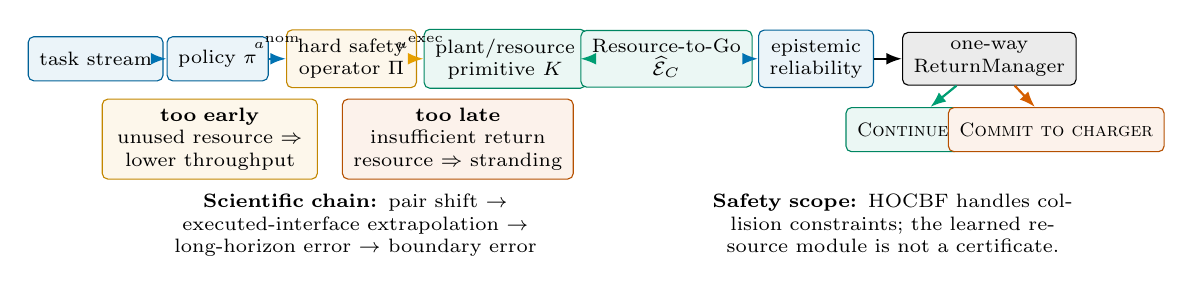
\begin{tikzpicture}[
  x=1cm,y=1cm,
  font=\scriptsize,
  box/.style={draw=#1!85!black,fill=#1!8,rounded corners=2pt,minimum height=0.56cm,align=center,inner xsep=4pt},
  arr/.style={-{Latex[length=2.0mm]},thick,draw=#1},
  note/.style={align=center,font=\scriptsize},
]
\definecolor{oiBlue}{HTML}{0072B2}
\definecolor{oiOrange}{HTML}{E69F00}
\definecolor{oiGreen}{HTML}{009E73}
\definecolor{oiVerm}{HTML}{D55E00}

\node[box=oiBlue,minimum width=1.25cm] (task) at (0,0) {task stream};
\node[box=oiBlue,minimum width=1.15cm] (pi) at (1.55,0) {policy $\pi$};
\node[box=oiOrange,minimum width=1.40cm] (filter) at (3.25,0) {hard safety\\operator $\Pi$};
\node[box=oiGreen,minimum width=1.55cm] (plant) at (5.20,0) {plant/resource\\primitive $K$};
\node[box=oiGreen,minimum width=1.45cm] (rtg) at (7.25,0) {Resource-to-Go\\$\widehat{\mathcal E}_C$};
\node[box=oiBlue,minimum width=1.35cm] (rel) at (9.15,0) {epistemic\\reliability};
\node[box=black,minimum width=1.85cm] (manager) at (11.35,0) {one-way\\ReturnManager};

\draw[arr=oiBlue] (task) -- (pi);
\draw[arr=oiBlue] (pi) -- node[above,font=\tiny] {$a^{\rm nom}$} (filter);
\draw[arr=oiOrange] (filter) -- node[above,font=\tiny] {$u^{\rm exec}$} (plant);
\draw[arr=oiGreen] (plant) -- (rtg);
\draw[arr=oiBlue] (rtg) -- (rel);
\draw[arr=black] (rel) -- (manager);

\node[box=oiGreen,minimum width=1.20cm] (cont) at (10.25,-0.90) {\textsc{Continue}};
\node[box=oiVerm,minimum width=1.55cm] (ret) at (12.20,-0.90) {\textsc{Commit to charger}};
\draw[arr=oiGreen] (manager) -- (cont);
\draw[arr=oiVerm] (manager) -- (ret);

\node[box=oiOrange,text width=2.45cm,minimum height=0.72cm] (early) at (1.45,-1.02) {\textbf{too early}\\unused resource $\Rightarrow$ lower throughput};
\node[box=oiVerm,text width=2.65cm,minimum height=0.72cm] (late) at (4.60,-1.02) {\textbf{too late}\\insufficient return resource $\Rightarrow$ stranding};
\node[note,anchor=north west,text width=6.45cm] at (-0.05,-1.60) {\textbf{Scientific chain:} pair shift $\to$ executed-interface extrapolation $\to$ long-horizon error $\to$ boundary error};
\node[note,anchor=north west,text width=5.65cm] at (7.15,-1.60) {\textbf{Safety scope:} HOCBF handles collision constraints; the learned resource module is not a certificate.};
\end{tikzpicture}
}
  \captionof{figure}{\textbf{Return decisions depend on the executed closed loop.} The task policy proposes \(a^{\rm nom}\), the hard safety operator produces \(u^{\rm exec}\), and the shared plant/resource primitive determines charger Resource-to-Go. The learned module estimates this requirement and may abstain when epistemic reliability is poor; it does not certify collision safety. Committing too early reduces throughput, while committing after the available-resource boundary risks stranding.}
  \label{fig:overview}
\end{center}

State of charge and charger distance are tempting decision variables, but neither specifies the resource required by the trajectory that will actually be executed. A learned policy proposes a nominal action, a safety operator may replace that action, and the plant then realizes motion and resource use. Thus the relevant chain is
\(
\pi\!\to\! a^{\mathrm{nom}}\!\to\!\Pi\!\to\!u^{\mathrm{exec}}\!\to\!K\!\to\!\RtoGo
\),
where \(\RtoGo\) is charger Resource-to-Go. An obstacle that activates the filter can make two equally distant states require different maneuvers and resources. Figure~\ref{fig:overview} states the resulting decision problem and the scope of each component.

Existing work addresses parts of this chain. Trajectory-energy models estimate consumption and risk \citep{choudhry2021cvar}, and predictive resource-safety networks place a learned override above task policies \citep{guo2020predictive}; constrained and distributional RL optimize policies under resource, expected-cost, or risk-sensitive constraints \citep{qin2021density,achiam2017cpo,liu2022cvpo,kim2023sdac}; and policy-conditioned or compositional world models adapt predictions across policies or structured environments \citep{chen2024pcm,zhao2022howm,wang2025wm3c}. Ensembles and selective prediction estimate when a predictor may fail \citep{lakshminarayanan2017ensembles,geifman2019selectivenet}. Yet none of these pieces by itself identifies what must be covered when a separately queryable safety operator rewrites actions, or when a prediction error changes an irreversible return decision.

Our first insight is that \emph{pair novelty is not equivalent to executed-interface extrapolation}. An unseen pair \((\pi,\Pi)\) need not be statistically novel at the primitive interface if its induced \((x,u^{\rm exec})\) occupancy is identified. Conversely, observing each policy and each safety operator somewhere does not identify a target pair that reaches an uncovered executed interface. Our second insight is decision-theoretic: global Resource-to-Go error and mission-critical error are different. Under a threshold ReturnManager, bounded estimation error changes a decision only near the return boundary, and underestimation in this band is the direct route to late commitment.

We therefore study executed-interface Resource-to-Go, not a nominal-action energy label. We establish a paired identification/non-identification result, give an assumption-explicit finite-horizon transport bound with a proper stochastic-shortest-path truncation term, and prove return-boundary stability. The practical framework compares direct temporal-difference prediction, policy-conditioned and executed-action world models, and epistemic ensembles under a common irreversible ReturnManager. A more structured reliability mechanism is retained only if these simpler models fail a predeclared gate.

Our contributions are:
\begin{itemize}[leftmargin=*,topsep=2pt,itemsep=1pt]
  \item a formal executed-interface object that separates unseen pair identity from the support actually needed to identify charger Resource-to-Go;
  \item identification, impossibility, long-horizon error, and return-boundary results whose assumptions explicitly separate coverage from smoothness;
  \item a falsifiable protocol linking prediction error to return decisions through matched-support, matched-horizon, risk--coverage, and paired battery-cycle evaluations; and
  \item \resultpending{EMPIRICAL CLAIMS} an evidence slot for testing whether interface extrapolation and hitting horizon predict Resource-to-Go failure, and whether reliable estimates improve the stranding--throughput frontier.
\end{itemize}

\section{Related Work}
\label{sec:related}

\paragraph{Energy prediction and return sufficiency.}
Flight-energy models combine trajectory context with learned power prediction and can propagate uncertainty into pre-flight risk measures \citep{choudhry2021cvar}. Persistent-robot work also schedules UAV charging rendezvous \citep{mathew2015rendezvous}, while predictive resource-safety networks hierarchically override task policies using forecasts of future resource levels \citep{guo2020predictive}. Battery-persistification filters keep a state-of-charge lower bound forward invariant under a nominal task controller \citep{notomista2018persistification}, with energy-sufficiency extensions for unknown environments \citep{fouad2023energysufficiency}; later work criticizes this line for relying on fixed state-of-charge thresholds and simplified energy models. Reach-avoid safety filters can instead return an agent to a charging target within a deadline \citep{begzadic2025backtobase}, but they switch on a learned state value without a battery-conditioned return requirement or a statistical account of the decision. End-to-end learning can also fold recharging into a coverage policy on a discrete grid \citep{theile2023recharge}, and recent warehouse studies report that context-dependent charging decisions beat fixed-threshold rules on discrete routing tasks \citep{shaji2026orderpickers}; the reliability literature provides optimal abort-threshold theory for analytic reliability models, not for learned closed loops. These works make the closest practical case for our problem. Our narrower distinction is that the return requirement is generated online by a task policy composed with a separately queryable intervention operator; we ask what executed interface must be covered and evaluate errors at the downstream irreversible decision. Thus geometric distance alone is inadequate, but a learned hierarchy alone is not our claimed novelty.

\paragraph{Constrained and distributional control.}
CMDP methods constrain expected costs during policy optimization \citep{achiam2017cpo,liu2022cvpo}; density-constrained RL includes an electric-vehicle charging case with remaining-energy and station-capacity constraints \citep{qin2021density}; distributional methods learn return or cost distributions for risk-sensitive decisions \citep{bellemare2017distributional,dabney2018iqn,yang2019fqf,kim2023sdac}. Reach-avoid RL learns reachability--avoidance values for safe return to a target set \citep{hsu2021reachavoid} and has been extended to minimum-cost objectives under deterministic \citep{so2024rcppo} and probabilistic \citep{pan2026rapcpo} formulations. Recovery-oriented frameworks separate task and recovery policies behind a learned safety critic \citep{thananjeyan2021recovery}, or threshold intervention using a cost action-value under the backup semantics \citep{wagener2021sailr}. Feasibility-oriented methods learn the largest persistently safe set \citep{yu2022rcrl}, augment the state with a remaining safety budget \citep{sootla2022saute}, or synthesize strategies over formal battery and reload-state models \citep{blahoudek2020consumption}. These methods motivate our end-to-end baselines, but do not eliminate the modular question. We deliberately retain a hard, independently queryable collision filter and ask whether an already deployed task policy should continue or irreversibly return. In the present deterministic simulator, distributional critics are comparisons or future extensions, not evidence for physical q95/q99 tails.

\paragraph{World models under policy and composition shift.}
Offline model-based RL controls model exploitation through uncertainty or pessimism \citep{yu2020mopo,kidambi2020morel,yu2021combo}. PCM goes closer by adapting finite-capacity dynamics models to a target policy's occupancy \citep{chen2024pcm}, while compositional world models exploit object or causal structure \citep{zhao2022howm,wang2025wm3c}. Our distinction is the interface: the safety operator maps nominal actions into executed actions before the shared primitive is invoked. Consequently, observing component identities does not imply coverage of the target executed occupancy. Our positive result is only identification under that coverage; it is not a finite-sample guarantee or a generic compositional world-model claim.

\paragraph{Uncertainty, abstention, and hard filters.}
Deep Ensembles are a strong, simple epistemic baseline \citep{lakshminarayanan2017ensembles}, but uncertainty quality can deteriorate under dataset shift \citep{ovadia2019uncertainty}. Selective prediction trades coverage for accepted risk \citep{geifman2019selectivenet}; conformal regression supplies marginal coverage under exchangeability, or under covariate shift with correct weighting assumptions \citep{romano2019cqr,tibshirani2019covshift}. We therefore evaluate risk--coverage rather than presume calibration transfers to a new composition. Recent work learns stoppability or contingency values---whether a safe stop or a diversion to any of several back-up targets remains feasible---from data \citep{long2026stoppability,lishkova2026contingencies}; these estimate reach--avoid feasibility for a fixed maneuver, without conditioning on remaining battery or committing to a return decision with trajectory-level risk accounting. Separately, HOCBFs and safety filters target forward-invariant collision constraints \citep{xiao2022hocbf,lavanakul2024safetyfilters}. They remain the hard-safety authority; Resource-to-Go reliability only informs when to return.

\section{Problem Setup}
\label{sec:problem}

Let \(\mathsf X,\mathsf A,\mathsf U\) be standard Borel state, nominal-action, and executed-action spaces. A task policy \(\pi(da\mid x)\) proposes \(a\), and a queryable safety operator \(K_\Pi(du\mid x,a)\) produces \(u\). The shared plant/resource primitive is
\[
K(dx',dc\mid x,u),\qquad c\in[0,c_{\max}],
\]
so the executed closed-loop kernel is
\begin{equation}
Q^{\pi,\Pi}_K(dx',dc\mid x)
=\int\pi(da\mid x)\int K_\Pi(du\mid x,a)K(dx',dc\mid x,u).
\label{eq:closedloop}
\end{equation}
For a measurable charger set \(G_C\), define the hitting time \(T_C=\inf\{t\geq0:x_t\in G_C\}\) and Resource-to-Go
\begin{equation}
E_C=\sum_{t=0}^{T_C-1}c_t, \qquad \mathcal Z_C(x)=\mathcal L(E_C\mid x_0=x).
\label{eq:rtg}
\end{equation}
The charger is absorbing with zero subsequent cost. We assume a proper stochastic shortest path (SSP): \(T_C<\infty\) almost surely and \(\mathbb E[T_C]<\infty\) for states under study.

At a return check, \(b_t\) is remaining resource and \(m\geq0\) is a reserve. The decision is \(d_t\in\{\continueaction,\returnaction\}\), with \(\returnaction\) absorbing for the remainder of the battery cycle. Given a requirement \(U_t\), the oracle decision is \(d_t^\star=\mathbf{1}\{b_t\leq U_t+m\}\); the deployed manager replaces \(U_t\) by \(\widehat U_t\), or fails closed when the prediction is rejected.

\paragraph{Probability and safety semantics.}
The present simulator has deterministic dynamics conditional on its information state. Accordingly, the learned target is point Resource-to-Go and the uncertainty object is epistemic error from finite data or extrapolation. We do not interpret ensemble percentiles as physical aleatoric q95/q99. Collision avoidance is certified, when its assumptions hold, by the HOCBF layer; the learned Resource-to-Go module provides no collision or energy-safety certificate.

\begin{remark}[Stochastic extension]
With a declared stochastic primitive and repeated fixed-condition rollouts, \(\mathcal Z_C(x)\) may be a non-degenerate conditional law. All tail or conformal claims would then require a new calibration audit under the deployed composition; this extension is outside the current empirical claim set.
\end{remark}

\section{What Must Be Covered?}
\label{sec:interface}

For the target composition \((\pi^\star,\Pi^\star)\), let \(d_t^\star\) denote its occupancy over executed interfaces \((x_t,u_t)\) before charger arrival. Let \(\mathcal K(\mathcal D)\) be primitive kernels observationally compatible with the source data. The following paired result separates component identity from the interface that determines future resource.

\begin{theorem}[Executed-interface identification]
\label{thm:identification}
Assume: (i) \(\pi^\star\) and \(K_{\Pi^\star}\) are queryable; (ii) the primitive \(K\) is shared across source and target compositions; (iii) every \(\widetilde K\in\mathcal K(\mathcal D)\) agrees with the true primitive \(K_0\), up to \(d_t^\star\)-null sets, on each target executed interface before \(T_C\); and (iv) the proper-SSP assumptions in Section~\ref{sec:problem} hold. Then the target finite-dimensional path law up to charger arrival, and hence \(\mathcal Z_C^{\pi^\star,\Pi^\star}(x)\), are uniquely identified, even if the pair \((\pi^\star,\Pi^\star)\) never generated a source trajectory.
\end{theorem}

The proof composes the queryable kernels in Equation~\eqref{eq:closedloop}, applies uniqueness of the induced path measure, and passes from finite truncated sums to \(E_C\) in \(L^1\). It is an identification statement, not a learning rate.

\begin{proposition}[Non-identification outside interface support]
\label{prop:nonident}
Suppose a measurable interface region \(B\subseteq\mathsf X\times\mathsf U\) has zero probability under every source trajectory but is reached before the charger with positive target probability. If the model class permits two bounded resource kernels that agree outside \(B\) and differ on \(B\), no source-observation-only estimator can uniformly identify the target Resource-to-Go law.
\end{proposition}

The construction makes the two primitives observationally equivalent on all source data and assigns different terminal costs at the first target visit to \(B\). Additional known physics can enable extrapolation, but must be stated as structure; coverage of policy and filter \emph{identities} alone is insufficient. Full statements and proofs are in Appendix~\ref{app:proofs}.

\section{From Interface Error to Return Error}
\label{sec:theory}

Identification does not quantify finite-sample error. For a finite horizon \(H\), compare the true primitive \(K\) with \(\widehat K\) while querying the same \(\pi\) and \(K_\Pi\). At each \((x,u)\), suppose a measurable one-step coupling of \((x',c)\) and \((\widehat x',\widehat c)\) exists, and learned continuation laws are \(L_{t+1}\)-Lipschitz in \(W_1\). Define
\[
\epsilon_t(x,u)=\mathbb E\big[|c-\widehat c|+L_{t+1}d(x',\widehat x')\big].
\]

\begin{theorem}[Occupancy-weighted finite-horizon transport]
\label{thm:transport}
Under the coupling and continuation regularity above,
\begin{equation}
W_1(\mathcal Z_{0:H}(x_0),\widehat{\mathcal Z}_{0:H}(x_0))
\leq\sum_{t=0}^{H-1}\mathbb E_{(x_t,u_t)\sim d_t^{\pi,\Pi,K}}[\epsilon_t(x_t,u_t)].
\label{eq:transport}
\end{equation}
Moreover, the proper SSP gives
\begin{equation}
W_1(\mathcal Z_C(x),\mathcal Z_{C,H}(x))
\leq c_{\max}\mathbb E[(T_C-H)_+]\to0.
\label{eq:truncation}
\end{equation}
\end{theorem}

Coverage alone does not imply Equation~\eqref{eq:transport}: continuation regularity may fail near discontinuous safety-filter active sets. The bound instead motivates two empirical variables---executed-interface extrapolation and hitting horizon---and requires both to be controlled in the experiment.

Finally, let the oracle and learned threshold decisions be
\(d^\star=\mathbf{1}\{b\leq U+m\}\) and
\(\widehat d=\mathbf{1}\{b\leq\widehat U+m\}\).

\begin{theorem}[Return-boundary stability]
\label{thm:boundary}
If \(|\widehat U-U|\leq\varepsilon\), then
\begin{equation}
d^\star\neq\widehat d\quad\Longrightarrow\quad |b-m-U|\leq\varepsilon.
\label{eq:boundary}
\end{equation}
\end{theorem}

Thus error can alter the threshold decision only within an \(\varepsilon\)-band around the boundary. This does not make global MAE irrelevant, nor imply that every disagreement causes stranding; it identifies where underestimation becomes decision-critical. Appendix~\ref{app:proofs} includes the proofs, decision-check overshoot condition, and task-plus-return risk allocation.

\section{A Modular Return Framework}
\label{sec:method}

The framework deliberately separates prediction, reliability, and authority.

\paragraph{Executed-interface Resource-to-Go.}
Training tuples expose the state, nominal action, executed action, realized resource, next state, composition identifier, and charger termination. We compare: (i) direct Monte-Carlo regression to realized charger cost; (ii) temporal-difference Resource-to-Go; (iii) PCM conditioned on the nominal policy; (iv) PCM with the executed interface; and (v) an executed-action world model rolled out through the queryable target \(\pi\) and \(\Pi\). All model-based methods receive the same target-component queries and executed-action information when applicable.

\paragraph{Epistemic reliability.}
A bootstrap Deep Ensemble supplies the default dispersion score. Thresholds are selected only on source/calibration compositions and evaluated as risk--coverage curves on held-out pairs. Rejection never becomes an unearned safety claim: the manager takes a predeclared conservative action when coverage is denied. Weighted conformal calibration is optional only if the required density-ratio assumptions and effective sample size are audited.

\paragraph{One-way ReturnManager.}
At fixed decision intervals, the manager commits when \(b_t\leq\widehat U_t+m\). Once committed, productive tasks cannot resume until charging completes. A conservative margin or fail-closed decision absorbs epistemic rejection; a separate check-interval reserve addresses resource spent between decisions. HOCBF continues to modify nominal navigation actions during both productive and return phases.

\paragraph{Gated candidate: SIRP.}
Support-Informed Reliability Prediction (SIRP) is \emph{not} part of the confirmed method. It may combine local executed-interface support, predicted hitting horizon, and ensemble disagreement only if the executed-world-model ensemble fails the predeclared risk--coverage gate and the added features explain residual severe underestimation. Otherwise it is removed in favor of the simpler ensemble baseline.

\section{Experimental Protocol}
\label{sec:experiments}

The evaluation is organized by falsifiable research questions rather than implementation stages. The primary domain is continuous UAV delivery with a separately trained navigation policy and HOCBF collision filter; a second domain/filter family is required for a generality claim. Current simulator outcomes are deterministic conditional on the information state.

\paragraph{RQ1: Is perfect Resource-to-Go useful?}
Before learning a predictor, an oracle manager uses simulator-exact charger cost under the same navigation and return code. It must improve completed tasks per battery cycle by at least 5\% at a matched stranding ceiling relative to tuned state-of-charge and distance--energy rules. This is a predeclared practical-relevance gate, not a significance threshold; the full effect and its interval are reported, and sensitivity to the gate is retained. Failure closes the downstream return-decision claim.

\paragraph{RQ2: Pair identity or executed-interface extrapolation?}
We use leave-one-pair-out compositions over policies and safety operators. Test sets cross seen/unseen pairs with low/high executed-interface extrapolation, while matching charger hitting-horizon distributions. Direct, TD, PCM-Nominal, PCM-Executed, executed-WM, executed-WM Ensemble, and Oracle receive fair component access. The mechanism claim requires error to track interface risk after controlling for pair identity and horizon.

\paragraph{RQ3: Can reliability detect future failures?}
On held-out compositions, we measure accepted-set MAE, severe underestimation, risk--coverage, and area under the risk--coverage curve (AURC). Ensemble disagreement and simple $k$NN interface distance are mandatory baselines. SIRP is evaluated only if its gate in Section~\ref{sec:method} opens. No threshold is tuned on test compositions.

\paragraph{RQ4: Does reliability improve decisions?}
All estimators feed the same one-way ReturnManager. Comparisons include state-of-charge thresholds, distance--energy, a receding-horizon planner using the same declared plant/resource primitive, a Predictive-Safety-Network-style resource-safety head, a direct high-level continue/return switcher, direct Resource-to-Go, PCM, executed-WM, ensemble-conservative return, the gated candidate (if retained), and Oracle. The matched end-to-end track includes CPO/CVPO/SDAC and DCRL when its density-constraint semantics can be made task-equivalent; otherwise the incompatibility is reported rather than hidden. The main outcome is the paired stranding--throughput frontier; secondary outcomes are charger return success, unused charger-arrival resource, premature return, and tasks per simulated hour.

\paragraph{RQ5: Does the phenomenon generalize?}
The full pair/support/horizon regime is repeated in a second domain or with a materially different safety-operator family. Without this replication, claims remain scoped to the primary simulator.

\paragraph{Statistics and stopping rules.}
Every frontier point starts with at least 100 independent battery cycles, but the final count is preregistered from the precision needed at the declared stranding ceiling; 100 cycles alone cannot substantiate a one-percent-level rare-event claim. Rare-event stranding receives Wilson intervals; method differences use paired cycle-level bootstrap intervals under common task and disturbance seeds. Navigation requires three passing seeds before it can support downstream claims. Fail-closed gates stop the pipeline after navigation, held-out battery calibration, Oracle headroom, prediction pilot, or generality failure. Appendix~\ref{app:experimental} records splits, fairness controls, and the complete baseline matrix.

\section{Results: Pre-Registered Evidence Slots}
\label{sec:results}

No downstream experiment is promoted to a paper result in this pre-results draft. Each slot below maps to the repository completion ledger and has an explicit claim gate.

\begin{center}
\centering
\small
\captionof{table}{Main result slots. Empty cells are intentional: values will be inserted only from completed, audited artifacts. Arrows indicate desired directions, not outcomes.}
\label{tab:result-slots}
\begin{tabular}{p{0.25\linewidth}p{0.37\linewidth}p{0.26\linewidth}}
\toprule
Question & Primary metric & Current status \\
\midrule
Navigation readiness & success, path ratio, contacts & \textcolor{BrickRed}{\textbf{PENDING: NAV}} \\
Oracle headroom & tasks/cycle at fixed stranding & \textcolor{BrickRed}{\textbf{PENDING: ORACLE}} \\
Prediction pilot & MAE, boundary underestimation & \textcolor{BrickRed}{\textbf{PENDING: PILOT}} \\
Failure mechanism & pair vs. interface vs. horizon & \textcolor{BrickRed}{\textbf{PENDING: MECHANISM}} \\
Selective reliability & AURC, severe underestimation & \textcolor{BrickRed}{\textbf{PENDING: UQ}} \\
Return decision & stranding--throughput frontier & \textcolor{BrickRed}{\textbf{PENDING: PARETO}} \\
Generality & replicated regimes & \textcolor{BrickRed}{\textbf{PENDING: REPL.}} \\
End-to-end alternative & matched-budget CMDP track & \textcolor{BrickRed}{\textbf{PENDING: CMDP}} \\
\bottomrule
\end{tabular}
\end{center}

The planned reporting order is deliberately causal: establish navigation and oracle headroom; test the pair/interface/horizon mechanism; evaluate accepted-risk calibration; then connect predictions to paired mission outcomes. Appendix~\ref{app:result-sheets} contains fill-in tables with provenance fields. Historical short runs and a failed navigation gate are retained as engineering evidence but cannot fill these slots.

\section{Limitations and Discussion}
\label{sec:limitations}

The theory has sharp but restrictive scope. Target-interface agreement is an identification assumption, not an observable finite-sample certificate. The transport result separately requires a one-step coupling and Lipschitz continuation laws, which can fail at discontinuous safety-filter active-set changes. Small Wasserstein error does not imply stable high quantiles without local distributional regularity. In the current deterministic simulator, physical tail-risk language would therefore be misleading.

The empirical claim is also conditional. If exact Resource-to-Go has no headroom over simple heuristics, the problem may not warrant a learned manager in this domain. If executed-WM plus Deep Ensemble explains failures, SIRP should be deleted. If only the primary UAV simulator exhibits the mechanism, the conclusion must remain domain-specific. Finally, the learned module does not guarantee charger reachability or collision avoidance; it supports a stopping decision while HOCBF retains collision-safety authority.

These limitations suggest a broader interpretation. The useful abstraction is not “battery prediction,” but a stopping problem in which a resource forecast is evaluated through the interface actually executed and through the decision boundary it can cross. The same analysis may apply to robots returning for charge, tools, data upload, or thermal recovery, but such transfer is a hypothesis until replicated.

\section{Conclusion}
\label{sec:conclusion}

We formulate return-to-replenishment as a closed-loop prediction-and-stopping problem. The executed interface, rather than policy--operator pair identity alone, determines whether a target Resource-to-Go law is identified; local model error can accumulate with the charger hitting horizon; and bounded requirement error affects a threshold decision only near the return boundary. These results motivate a simple modular hierarchy: executed-interface prediction, empirically validated epistemic rejection, and a one-way ReturnManager, with hard collision safety kept separate. \resultpending{EMPIRICAL VALIDATION} will determine whether this mechanism improves the stranding--throughput frontier and generalizes beyond the primary simulator.


\bibliography{references}
\bibliographystyle{iclr2027_conference}

\clearpage
\appendix
\section{Proofs and Technical Scope}
\label{app:proofs}

\subsection{Common assumptions}

State, nominal-action, executed-action, and resource spaces are standard Borel; the charger set is measurable. The target policy and safety operator are known/queryable Markov kernels. The plant/resource primitive receives the executed action and is shared across the compositions being compared. The charger is absorbing at zero subsequent cost. For every initial state considered, the charger hitting time is almost surely finite and integrable, and \(0\leq c_t\leq c_{\max}\).

\subsection{Proof of Theorem~\ref{thm:identification}}

Equation~\eqref{eq:closedloop} defines a Markov kernel by measurability of the component kernels. Fix any primitive \(\widetilde K\) observationally compatible with source data. By target-interface identification, \(\widetilde K\) and \(K_0\) agree almost everywhere under every true target executed occupancy before charger arrival. Integrating the same queryable \(\pi^\star\) and \(K_{\Pi^\star}\) therefore yields equal closed-loop kernels at target-reached states, up to path-law null sets.

Starting from \(\delta_x\), Ionescu--Tulcea gives a unique measure on finite path cylinders. Induction on cylinder length shows that \(K_0\) and \(\widetilde K\) induce the same finite path law: their current marginals agree, and the next conditional kernels agree almost everywhere under this common marginal. For each \(H\), the truncated sum \(E_{C,H}\) is a measurable function of a finite path prefix and its pushforward law is therefore identified. Finally,
\[
0\leq E_C-E_{C,H}\leq c_{\max}(T_C-H)_+,
\]
whose expectation converges to zero by integrability of \(T_C\). Thus \(E_{C,H}\to E_C\) in \(L^1\), hence in distribution, and the unique truncated laws identify \(\mathcal Z_C\). No source trajectory from the complete target pair is used. \(\square\)

\subsection{Proof of Proposition~\ref{prop:nonident}}

Choose \(r_1\neq r_2\) in \([0,c_{\max}]\). Let \(K_1\) and \(K_2\) agree outside \(B\). On \(B\), both transition to a fixed charger state but incur \(r_1\) and \(r_2\), respectively. Since all source occupancies assign zero probability to \(B\), the complete source-data laws under \(K_1\) and \(K_2\) coincide. Any estimator based only on source observations has the same output distribution in both worlds. Before the first target visit \(\tau_B\), the target path laws also coincide; on the positive-probability event \(\tau_B<T_C\), they then incur different terminal resource. The target Resource-to-Go laws differ, so no common estimator can uniformly identify both. \(\square\)

\subsection{Proof of Theorem~\ref{thm:transport}}

Let \(e_t(x)=W_1(\mathcal Z_{t:H}(x),\widehat{\mathcal Z}_{t:H}(x))\) and \(e_H=0\). At a common state \(x\), draw the same \(a\sim\pi(\cdot\mid x)\) and \(u\sim K_\Pi(\cdot\mid x,a)\), then couple primitive outcomes. By the triangle inequality and continuation-law Lipschitzness,
\[
W_1\!\left(\mathcal Z_{t+1:H}(x'),\widehat{\mathcal Z}_{t+1:H}(\widehat x')\right)
\leq e_{t+1}(x')+L_{t+1}d(x',\widehat x').
\]
Adding the coupled immediate resources yields
\[
e_t(x)\leq \mathbb E_{a,u}[\epsilon_t(x,u)]
+\mathbb E_{x'\sim Q_K^{\pi,\Pi}(\cdot\mid x)}[e_{t+1}(x')].
\]
Unrolling under the true target kernel gives Equation~\eqref{eq:transport}. For truncation, couple \(E_C\) and \(E_{C,H}\) on the same trajectory. The tail is bounded by \(c_{\max}(T_C-H)_+\), and dominated convergence proves Equation~\eqref{eq:truncation}. \(\square\)

\subsection{Proof of Theorem~\ref{thm:boundary}}

Let \(\theta=U+m\) and \(\widehat\theta=\widehat U+m\). If the two indicators differ, \(b\) lies between their thresholds, including the appropriate endpoint. Hence
\[
|b-\theta|\leq|\widehat\theta-\theta|=|\widehat U-U|\leq\varepsilon,
\]
which is Equation~\eqref{eq:boundary}. \(\square\)

\subsection{Decision-interval overshoot}

Suppose accepted predictions satisfy
\(\Pr(E_{C,t}\leq U_t\mid\text{accepted at }t)\geq1-\delta\).
Let \(D_s=b_s-U_s\), and assume that between checks
\[
(b_{t-1}-b_t)+(U_t-U_{t-1})\leq\Delta_{\rm check}.
\]
If the one-way manager first commits at \(t\), then \(D_{t-1}>m\). For \(m\geq\Delta_{\rm check}\),
\(D_t>D_{t-1}-\Delta_{\rm check}>0\), so \(b_t>U_t\). Conditional on acceptance and excluding non-energy failure modes, exhaustion before charger arrival then has probability at most \(\delta\). This statement depends on calibration for the deployed composition and does not transfer collision-safety authority from HOCBF.

\subsection{Task-plus-return allocation}

For task resource \(E_T\) and return resource \(E_R\) on the same mission probability space, if
\(\Pr(E_T\leq U_T)\geq1-\delta_T\) and
\(\Pr(E_R\leq U_R)\geq1-\delta_R\), the union bound gives
\[
\Pr(E_T+E_R\leq U_T+U_R)\geq1-\delta_T-\delta_R,
\]
without independence. Thus adding two marginal q95 bounds supports only a 90\% lower bound by this argument; it does not support a 95\% joint claim.

\subsection{Explicit non-claims}

The theory does not show that ensemble variance or $k$NN distance equals the local transport error; that small \(W_1\) controls q95/q99; that component identity coverage implies target-interface identification; or that calibration survives arbitrary composition shift. Each is either an empirical question or requires additional assumptions.

\section{Complete Experimental Design}
\label{app:experimental}

\subsection{Gate chain and provenance}

The experiment order is navigation capability $\rightarrow$ battery calibration $\rightarrow$ Oracle headroom $\rightarrow$ frozen-policy prediction $\rightarrow$ closed-loop decision $\rightarrow$ second-domain/filter replication $\rightarrow$ matched end-to-end CMDP comparison. A downstream gate cannot be reported when an upstream gate fails. Every reported cell must record configuration, code revision, checkpoint, raw artifact path, seed list, sample count, and evaluation script.

\subsection{Composition split}

Let \(\{\pi_i\}_{i=1}^P\) and \(\{\Pi_j\}_{j=1}^F\) be frozen policies and safety operators. Leave-one-pair-out evaluation withholds complete pairs while retaining separately seen components where possible. Within each held-out pair, states are stratified by an interface-risk score computed only from source executed \((x,u)\) samples and by true charger hitting horizon. The primary factorial analysis crosses pair seen/unseen, interface low/high extrapolation, and horizon short/long. Reporting the marginal pair effect without these controls is forbidden.

\subsection{Prediction and decision baselines}

\begin{table}[t]
\centering
\small
\caption{Baseline information contract. ``Query'' means access to the frozen target component, not target outcomes.}
\label{tab:baselines}
\begin{tabular}{lcccc}
\toprule
Method & $a^{\rm nom}$ & $u^{\rm exec}$ & query $\pi,\Pi$ & reliability \\
\midrule
Distance $\times$ rate & no & no & no & no \\
Receding-horizon planner & no & yes & yes & explicit model \\
Predictive-safety head & optional & yes & no & learned safety score \\
Direct MC / TD & optional & yes & no & ensemble option \\
PCM-Nominal & yes & no & $\pi$ & ensemble option \\
PCM-Executed & yes & yes & $\pi,\Pi$ & ensemble option \\
Executed-WM & no & yes & $\pi,\Pi$ & no \\
Executed-WM Ensemble & no & yes & $\pi,\Pi$ & ensemble \\
SIRP candidate & no & yes & $\pi,\Pi$ & support+horizon+ensemble \\
Oracle & realized & realized & yes & exact simulator clone \\
CMDP/DCRL track & task state & environment & no & method-specific \\
\bottomrule
\end{tabular}
\end{table}


The Oracle uses the simulator's realized charger Resource-to-Go under a cloned information state and the same target policy/filter, without exposing future task rewards to learned methods. The receding-horizon planner may query the same frozen plant/resource primitive but not realized future task rewards; its horizon, compute budget, and terminal approximation are reported. The predictive-safety head adapts the future-resource hierarchy of \citet{guo2020predictive} to the single-agent setting and receives no privileged target outcome. The direct switcher observes the same high-level state available to the ReturnManager but does not receive oracle future resource. CMDP methods receive a matched interaction budget and are evaluated under the same mission starts; CPO, CVPO, SDAC, and DCRL are included when their constraint semantics can be matched, and any non-equivalence is stated. Their collision semantics are reported separately from HOCBF-filtered modular methods.

\subsection{Metrics}

Prediction metrics are MAE, RMSE, signed bias, underestimation rate and magnitude, boundary-weighted underestimation, horizon-stratified error, accepted-set risk, coverage, and AURC. Mission metrics are energy exhaustion/stranding, tasks per battery cycle, tasks per simulated hour, successful charger return, unused resource at arrival, premature return, and the paired stranding--throughput frontier. CRPS, pinball losses, and conditional coverage are disabled unless a future stochastic-environment gate establishes a non-degenerate conditional resource law.

\subsection{Statistical reporting}

For a binary event with \(k\) occurrences in \(n\) cycles, report the Wilson interval at the declared confidence level. Before evaluation, choose \(n\) from the desired upper-bound or half-width precision at the declared stranding ceiling; the minimum of 100 cycles is only a floor, not evidence that a rare-event target has been resolved. For paired method contrasts, resample cycles with their shared task seeds and report percentile bootstrap intervals, number of resamples, and the complete seed set. The 5\% Oracle gate is reported together with its continuous effect estimate and a sensitivity analysis. No claim is formed from one navigation seed or fewer than the preregistered cycle count per frontier point.

\section{Result Sheets}
\label{app:result-sheets}

\subsection{Prediction mechanism sheet}

\begin{center}
\centering
\small
\captionof{table}{Prediction results template. Every dash remains empty until the corresponding artifact passes audit.}
\begin{tabular}{lcccccc}
\toprule
Method & MAE$\downarrow$ & Bias$\to0$ & Under.$\downarrow$ & BW-under.$\downarrow$ & AURC$\downarrow$ & Provenance \\
\midrule
Distance $\times$ rate & -- & -- & -- & -- & -- & -- \\
Direct MC & -- & -- & -- & -- & -- & -- \\
TD Resource-to-Go & -- & -- & -- & -- & -- & -- \\
PCM-Nominal & -- & -- & -- & -- & -- & -- \\
PCM-Executed & -- & -- & -- & -- & -- & -- \\
Executed-WM & -- & -- & -- & -- & -- & -- \\
Executed-WM + Ensemble & -- & -- & -- & -- & -- & -- \\
SIRP (only if gate opens) & -- & -- & -- & -- & -- & -- \\
Oracle & -- & -- & -- & -- & -- & -- \\
\bottomrule
\end{tabular}
\end{center}

\newpage
\subsection{Decision sheet}

\begin{center}
\centering
\small
\captionof{table}{Return-decision results template at matched stranding ceilings or matched throughput.}
\begin{tabular}{p{0.23\linewidth}ccccc}
\toprule
Manager & Strand.$\downarrow$ & Tasks/cycle$\uparrow$ & Return$\uparrow$ & Unused$\downarrow$ & Source \\
\midrule
SOC thresholds & -- & -- & -- & -- & -- \\
Distance--energy & -- & -- & -- & -- & -- \\
Receding-horizon planner & -- & -- & -- & -- & -- \\
Predictive-safety head & -- & -- & -- & -- & -- \\
Direct switcher & -- & -- & -- & -- & -- \\
Direct Resource-to-Go & -- & -- & -- & -- & -- \\
Executed-WM ensemble & -- & -- & -- & -- & -- \\
Gated candidate & -- & -- & -- & -- & -- \\
Oracle & -- & -- & -- & -- & -- \\
CMDP track & -- & -- & -- & -- & -- \\
\bottomrule
\end{tabular}
\end{center}

\section*{AI Use Statement}
\label{sec:ai-use}

\textbf{Author rewrite and factual confirmation pending.} For the final submitted version, generative AI tools will be disclosed only as assisting literature search, citation verification, and reference formatting. All other research and manuscript content in the submitted version will be independently written and verified by the authors. After the author rewrite is complete, this statement must be changed to past tense and checked against the final submission before upload.

\end{document}
